\subsection{Osculating Plane/Circle \& B-Hat $\left(\hat{B}\right)$}
\noindent
The osculating plane in the plane containing $\vec{r}(t)$, $\hat{T}$ and $\hat{N}$. It is only defined when $\hat{N}\neq 0$. This means straight lines do not have an osculating plane.
The osculating circle lives in the osculating plane, is centered at $\vec{r}(t) + \frac{\hat{N}(t)}{\kappa(t)}$, and has radius $\frac{1}{\kappa(t)}$.
The tangent line at $\vec{r}(t)$ is also tangent to the osculating circle because both points have the same curvature.

\begin{figure}[H]
	\label{osculating_plane_circle}
	\centering
	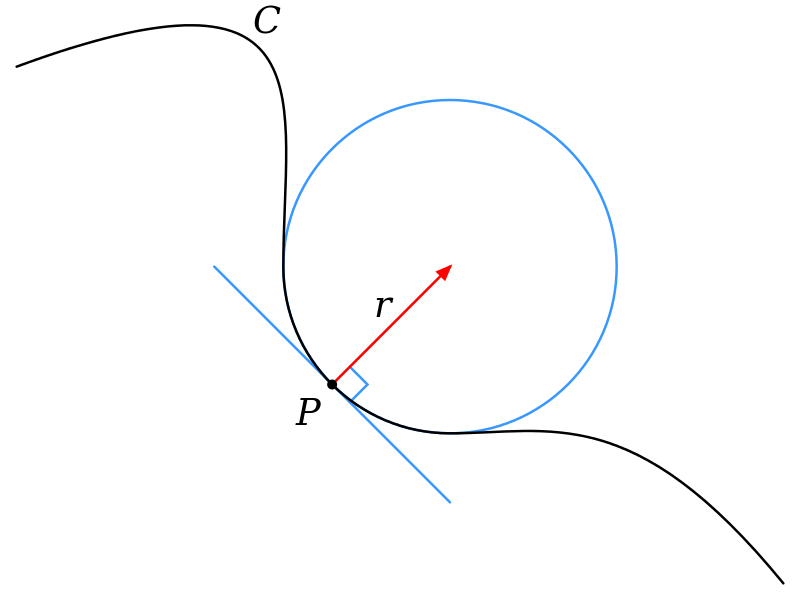
\includegraphics[width = 0.33\textwidth]{./Images/vectorValuedFunctions/osculatingCircle.png}
	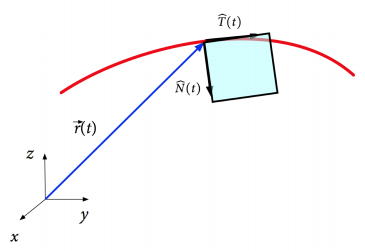
\includegraphics[width = 0.33\textwidth]{./Images/vectorValuedFunctions/osculatingPlane.png}
	\caption{Osculating circle and plane}
\end{figure}

\noindent
The vector that is normal to the plane is 
\begin{equation*}
	\hat{B}(t) = \hat{T}\times\hat{N},
\end{equation*}
which is called the ``binormal'' vector because it is perpendicular to both $\hat{T}$ and $\hat{N}$.
Together, $\hat{T}$, $\hat{N}$, and $\hat{B}$ form the Frenet Serret Frame, also called the TNB frame.

\begin{figure}[H]
	\label{osculating_plane_circle}
	\centering
	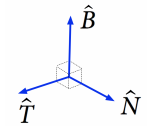
\includegraphics[width = 0.33\textwidth]{./Images/vectorValuedFunctions/TNB1.png}
	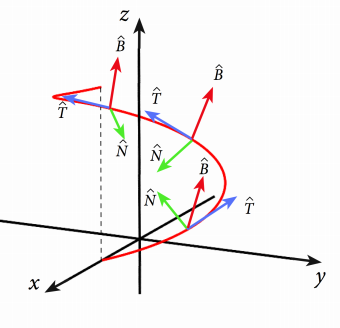
\includegraphics[width = 0.5\textwidth]{./Images/vectorValuedFunctions/TNB2.png}
	\caption{TNB frame}
\end{figure}

\noindent
We can write the equation for the osculating plane as
\begin{equation*}
	\hat{B}(t)\cdot\left(\langle x,y,z\rangle - \vec{r}(t)\right) = 0.
\end{equation*}